\documentclass[12pt]{article}

% Dimensões oficiais: 90 cm x 120 cm (padrão oficial pôster ABNT / UFABC)
\usepackage[paperwidth=90cm, paperheight=120cm, top=22.8cm, bottom=9.5cm, left=2.5cm, right=2.5cm]{geometry}

\usepackage[utf8]{inputenc}
\usepackage[T1]{fontenc}
\usepackage{lmodern}
\renewcommand{\familydefault}{\sfdefault} % Fonte sem serifa moderna e altamente legível

\usepackage{tikz}
\usetikzlibrary{calc}
\usepackage{xcolor}
\usepackage{graphicx}
\usepackage{booktabs}
\usepackage{amsmath}
\usepackage{amssymb}
\usepackage{caption}
\usepackage{enumitem}
\usepackage{microtype}

% Cor institucional verde UFABC do modelo PPTX original (#006633)
\definecolor{ufabcgreen}{RGB}{0, 102, 51}

\pagestyle{empty}

% Estilo de títulos de seção idêntico ao modelo PPTX (caixa alta, negrito)
\newcommand{\postersection}[1]{%
  {\noindent\fontsize{36pt}{42pt}\selectfont\textbf{#1}}\par%
  \vspace{0.45cm}%
}

\begin{document}
\noindent
% -------------------------------------------------------------
% BANNERS ESTRUTURAIS DE FUNDO (CABEÇALHO E RODAPÉ)
% -------------------------------------------------------------
\begin{tikzpicture}[remember picture, overlay]
  % Top Header Green Box (x = 0 a 60 cm, y = 0 a -15 cm)
  \fill[ufabcgreen] (current page.north west) rectangle ++(60cm, -15cm);
  
  % Título do Projeto no Top Header
  \node[anchor=center, text=white, font=\bfseries\fontsize{34pt}{40pt}\selectfont, text width=56cm, align=center] 
    at ($(current page.north west) + (30cm, -7.5cm)$) 
    {AVALIAÇÃO DE TÉCNICAS DE EXTRAÇÃO DE CARACTERÍSTICAS PARA\\ RECONHECIMENTO DE USUÁRIOS PELA IMPRESSÃO DIGITAL};

  % Top Header White Box com Logos Institucionais (x = 60 a 90 cm, y = 0 a -15 cm)
  \fill[white] ($(current page.north west) + (60cm, 0)$) rectangle ++(30cm, -15cm);
  \node[anchor=center] at ($(current page.north west) + (67.5cm, -7.5cm)$) {
    
\includegraphics[height=11.5cm, keepaspectratio]{figures/logos/ufabc_logo.jpg}
  };
  \node[anchor=center] at ($(current page.north west) + (81.5cm, -7.5cm)$) {
    
\includegraphics[height=11.0cm, keepaspectratio]{figures/logos/uscs_logo.png}
  };

  % Bloco de Autoria e Afiliação (x = centralizado, y = -15.5 a -22.5 cm)
  \node[anchor=north, text width=85cm, align=center] at ($(current page.north) + (0, -15.5cm)$) {
    {\fontsize{26pt}{32pt}\selectfont \textbf{Thiago Fernandes Dias}\textsuperscript{1,2}, \textbf{Paulo Henrique Pisani}\textsuperscript{1} (Orientador), \textbf{Francisco de Assis Zampirolli}\textsuperscript{1} (Coorientador)}\\[0.28cm]
    {\fontsize{21pt}{26pt}\selectfont \textsuperscript{1}Centro de Matemática, Computação e Cognição (CMCC) -- Universidade Federal do ABC (UFABC)}\\[0.18cm]
    {\fontsize{19pt}{24pt}\selectfont \textsuperscript{2}Bolsista de Iniciação Científica (CNPq) $\cdot$ Santo André -- SP, Brasil}\\[0.18cm]
    {\fontsize{18pt}{23pt}\selectfont \texttt{\{thiago.dias, paulo.pisani, f.zampirolli\}@ufabc.edu.br}}
  };

  % Bottom Footer White Box - Área de Apoio (x = 0 a 11 cm, y = 0 a 9 cm a partir da base)
  \fill[white] (current page.south west) rectangle ++(11cm, 9cm);
  \node[anchor=north west, font=\bfseries\fontsize{24pt}{28pt}\selectfont] at ($(current page.south west) + (0.8cm, 8.5cm)$) {Apoio:};
  
  \node[anchor=center] at ($(current page.south west) + (3.0cm, 5.3cm)$) {
    
\includegraphics[height=3.6cm, width=4.4cm, keepaspectratio]{figures/logos/ufabc_small.jpeg}
  };
  \node[anchor=center] at ($(current page.south west) + (7.8cm, 5.3cm)$) {
    
\includegraphics[height=3.5cm, width=5.0cm, keepaspectratio]{figures/logos/uscs_logo.png}
  };
  \node[anchor=center] at ($(current page.south west) + (5.5cm, 2.0cm)$) {
    
\includegraphics[width=9.2cm, height=3.5cm, keepaspectratio]{figures/logos/cnpq_logo.jpeg}
  };

  % Bottom Footer Green Box com Títulos dos Congressos (x = 11 a 90 cm)
  \fill[ufabcgreen] ($(current page.south west) + (11cm, 0)$) rectangle ++(79cm, 9cm);
  \node[anchor=east, text=white, align=right] at ($(current page.south east) + (-2.0cm, 4.5cm)$) {
    {\fontsize{36pt}{42pt}\selectfont \textbf{XVI Encontro de Iniciação Científica}}\\[0.22cm]
    {\fontsize{21pt}{25pt}\selectfont \textbf{XIX Simpósio de Iniciação Científica da UFABC}}\\[0.12cm]
    {\fontsize{21pt}{25pt}\selectfont \textbf{21º Congresso de Iniciação Científica da USCS}}
  };
\end{tikzpicture}%
% -------------------------------------------------------------
% CORPO DO PÔSTER: LAYOUT DE DUAS COLUNAS VERTICALMENTE DISTRIBUÍDAS
% -------------------------------------------------------------
\begin{minipage}[t][87.5cm][s]{41.5cm}
  \fontsize{26.5pt}{36pt}\selectfont
  
  \postersection{OBJETIVOS}
  Este projeto tem como objetivo central \textbf{avaliar e comparar o desempenho de diferentes técnicas de extração de características para o reconhecimento de usuários pela impressão digital}.
  Os objetivos específicos compreendem:
  \begin{itemize}[leftmargin=1.5cm, itemsep=0.4cm, topsep=0.3cm]
    \item Avaliar arquiteturas de aprendizado profundo que extraem representações de tamanho fixo: vetorial unidimensional (\textit{DeepPrint}) e tensorial tridimensional densa multitarefa (\textit{FLARE});
    \item Contrastar os resultados com a abordagem clássica baseada em minúcias locais (\textit{Minutia Cylinder-Code} -- MCC);
    \item Analisar o impacto de técnicas de pré-processamento e realce de cristas (\textit{UNetEnh} e \textit{PriorEnh});
    \item Investigar a robustez dos modelos sob diferentes tecnologias de sensores (ópticos, capacitivos e térmicos) e sob ruídos severos.
  \end{itemize}

  \vfill
  \postersection{INTRODUÇÃO}
  A biometria por impressões digitais baseia-se na singularidade e perenidade dos padrões de cristas e vales formados na epiderme das pontas dos dedos. Em sistemas de identificação automatizada (\textit{Automated Fingerprint Identification Systems} -- AFIS), a forma de representação das características extraídas é um dos fatores mais determinantes tanto para a taxa de acerto quanto para a escalabilidade e tempo de resposta.

  Como capturas biométricas reais sofrem com rotação, translação, área de contato parcial, variações de pressão e ruídos severos de fundo, a extração de representações discriminativas e invariantes é indispensável. Historicamente, os métodos clássicos baseiam-se em minúcias (terminações e bifurcações de cristas). Embora acurados em imagens ópticas nítidas, exigem algoritmos de emparelhamento geométrico com elevado custo computacional. Recentemente, modelos profundos viabilizaram a geração de representações compactas de tamanho fixo, permitindo verificação em tempo real por métricas diretas de distância.

  \vfill
  \postersection{MATERIAIS E MÉTODOS}
  \textbf{Bases de Dados Avaliadas:}
  Foram utilizados os subconjuntos Parte A das competições \textit{Fingerprint Verification Competition} (FVC2000, FVC2002 e FVC2004) com sensores reais (DB1, DB2 e DB3), totalizando 800 imagens por base (100 dedos $\times$ 8 impressões). Adicionalmente, empregaram-se as bases ópticas da Neurotechnology: \textit{CrossMatch} (408 imagens) e \textit{DigitalPersona U.are.U} (520 imagens).

  \vspace{0.4cm}
  \begin{center}
    \fontsize{18pt}{24pt}\selectfont
    \captionof{table}{Especificação dos conjuntos de dados e tecnologias de sensores avaliados.}
    \vspace{0.2cm}
    \renewcommand{\arraystretch}{1.28}
    \setlength{\tabcolsep}{8.5pt}
    \begin{tabular}{lllcc}
      \toprule
      \textbf{Conjunto} & \textbf{Base} & \textbf{Tecnologia do Sensor} & \textbf{Resolução} & \textbf{Dimensões} \\
      \midrule
      FVC2000 & DB1-A & Óptico (Secure Desktop Scanner) & 500 dpi & $300 \times 300$ \\
              & DB2-A & Capacitivo (TouchChip) & 500 dpi & $256 \times 364$ \\
              & DB3-A & Óptico (DF-90) & 500 dpi & $448 \times 478$ \\
      \midrule
      FVC2002 & DB1-A & Óptico (TouchView II) & 500 dpi & $388 \times 374$ \\
              & DB2-A & Óptico (FX2000) & 569 dpi & $296 \times 560$ \\
              & DB3-A & Capacitivo (100 SC) & 500 dpi & $300 \times 300$ \\
      \midrule
      FVC2004 & DB1-A & Óptico (V300) & 500 dpi & $640 \times 480$ \\
              & DB2-A & Óptico (DigitalPersona U.are.U) & 500 dpi & $328 \times 364$ \\
              & DB3-A & Térmico (FingerChip) & 500 dpi & $300 \times 480$ \\
      \midrule
      Neurotech. & CrossMatch & Óptico (Verifier 300) & 500 dpi & $504 \times 480$ \\
                 & U.are.U & Óptico (U.are.U 4000) & 500 dpi & $440 \times 500$ \\
      \bottomrule
    \end{tabular}
  \end{center}

  \vfill
  \noindent\textbf{Métricas Biométricas:}
  A avaliação utilizou as taxas de falsa aceitação ($FMR$), falsa rejeição ($FNMR$) e a taxa de igual erro ($EER$), calculada no ponto operacional de mínima diferença $|FMR - FNMR|$.

  \vspace{0.35cm}
  \noindent\textbf{Arquiteturas Avaliadas:}
  \begin{itemize}[leftmargin=1.5cm, itemsep=0.4cm, topsep=0.3cm]
    \item \textbf{DeepPrint}: Rede convolucional profunda (CNN) com módulo Spatial Transformer Network (STN) para alinhamento intrínseco. Extrai um vetor unidimensional compacto de 512 dimensões via aprendizado multitarefa.
    \item \textbf{FLARE}: Modelo baseado na arquitetura FDRN (ResNet-34 adaptada com embeddings posicionais senoidais). Extrai um descritor denso tridimensional $f = (f_s \oplus f_m) \odot S$, preservando relações geométricas espaciais e suprimindo o fundo pela máscara de segmentação $S$.
    \item \textbf{MCC}: Técnica clássica baseada em minúcias locais que constrói cilindros 3D discretizando a vizinhança espacial e angular, alimentada pelo extrator de minúcias \textit{FingerNet}.
  \end{itemize}

  \vfill
  \noindent\textbf{Métrica de Similaridade Cosseno Normalizada (FLARE):}
  \begin{equation}
    M(q, g) = \frac{{f_q'}^T \cdot f_g'}{\|f_q \odot S_g\|_F \cdot \|f_g \odot S_q\|_F}
  \end{equation}
  O numerador efetua o produto interno restrito às regiões válidas de primeiro plano, enquanto o denominador normaliza pela norma de Frobenius da intersecção espacial compartilhada entre a consulta ($q$) e a referência ($g$).

  \vspace{0.35cm}
  \noindent\textbf{Modelos de Realce de Cristas:}
  Foram avaliadas as técnicas \textit{UNetEnh} (baseada em arquitetura U-Net para restauração de cristas) e \textit{PriorEnh} (modelo generativo com prior de orientação de cristas e difusão), comparando os resultados obtidos com e sem realce.

\end{minipage}\hfill
\begin{minipage}[t][87.5cm][s]{41.5cm}
  \fontsize{26.5pt}{36pt}\selectfont

  \postersection{RESULTADOS E DISCUSSÕES}
  A Tabela 2 apresenta o desempenho comparativo em $EER$ (\%) dos métodos base (sem realce) em todos os conjuntos avaliados. Os resultados evidenciam a superioridade marcante do \textbf{FLARE (Votação)}, que obteve $EER$ média geral de \textbf{0,64\%}.

  \vspace{0.4cm}
  \begin{center}
    \fontsize{16.5pt}{22pt}\selectfont
    \captionof{table}{$EER$ (\%) dos métodos base nos subconjuntos Parte A do FVC e bases da Neurotechnology.}
    \vspace{0.2cm}
    \renewcommand{\arraystretch}{1.25}
    \setlength{\tabcolsep}{9.5pt}
    \begin{tabular}{ll rrrr}
      \toprule
      \textbf{Edição / Origem} & \textbf{Base} & \textbf{DeepPrint} & \textbf{FLARE (Reg.)} & \textbf{FLARE (Vot.)} & \textbf{MCC} \\
      \midrule
      FVC2000 & DB1-A & 3,36 & 0,81 & 0,81 & 2,69 \\
       & DB2-A & 2,69 & 0,54 & 0,19 & 4,33 \\
       & DB3-A & 3,85 & 0,63 & 0,59 & 10,21 \\
      \cmidrule{2-6}
      \multicolumn{2}{l}{\textbf{Média FVC2000}} & \textbf{3,30} & \textbf{0,66} & \textbf{0,53} & \textbf{5,74} \\
      \midrule
      FVC2002 & DB1-A & 5,20 & 0,44 & 0,25 & -- \\
       & DB2-A & 8,19 & 0,62 & 0,69 & -- \\
       & DB3-A & 8,51 & 3,32 & 2,08 & -- \\
      \cmidrule{2-6}
      \multicolumn{2}{l}{\textbf{Média FVC2002}} & \textbf{7,30} & \textbf{1,46} & \textbf{1,01} & -- \\
      \midrule
      FVC2004 & DB1-A & 17,05 & 0,25 & 0,24 & -- \\
       & DB2-A & 5,27 & 1,44 & 0,87 & -- \\
       & DB3-A & 4,91 & 0,38 & 0,31 & -- \\
      \cmidrule{2-6}
      \multicolumn{2}{l}{\textbf{Média FVC2004}} & \textbf{9,08} & \textbf{0,69} & \textbf{0,47} & -- \\
      \midrule
      \multicolumn{2}{l}{\textbf{Média FVC}} & \textbf{6,56} & \textbf{0,94} & \textbf{0,67} & -- \\
      \midrule
      Neurotechnology & CrossMatch & 3,31 & 0,49 & 0,12 & 2,10 \\
       & U.are.U & 2,76 & 0,58 & 0,86 & 1,94 \\
      \cmidrule{2-6}
      \multicolumn{2}{l}{\textbf{Média Neurotechnology}} & \textbf{3,04} & \textbf{0,53} & \textbf{0,49} & \textbf{2,02} \\
      \midrule[\heavyrulewidth]
      \multicolumn{2}{l}{\textbf{Média Geral}} & \textbf{5,92} & \textbf{0,86} & \textbf{0,64} & -- \\
      \bottomrule
    \end{tabular}
  \end{center}

  \vfill
  A Figura 1 ilustra a distribuição das pontuações de similaridade para o subconjunto FVC2000 DB1-A e a base óptica CrossMatch. No FLARE, as pontuações de impostores (vermelho) concentram-se próximas a 0,2, enquanto usuários genuínos (verde) situam-se acima de 0,6, garantindo separação praticamente ideal. O MCC superou o DeepPrint em bases ópticas de alta qualidade (2,02\% contra 3,04\% na Neurotechnology e 2,69\% no FVC2000 DB1-A), mas degradou acentuadamente em sensores ruidosos (10,21\% no FVC2000 DB3-A).

  \vspace{0.4cm}
  \begin{center}
    % Linha 1: FVC2000 DB1-A
    \begin{minipage}[b]{0.32\linewidth}
      \centering
      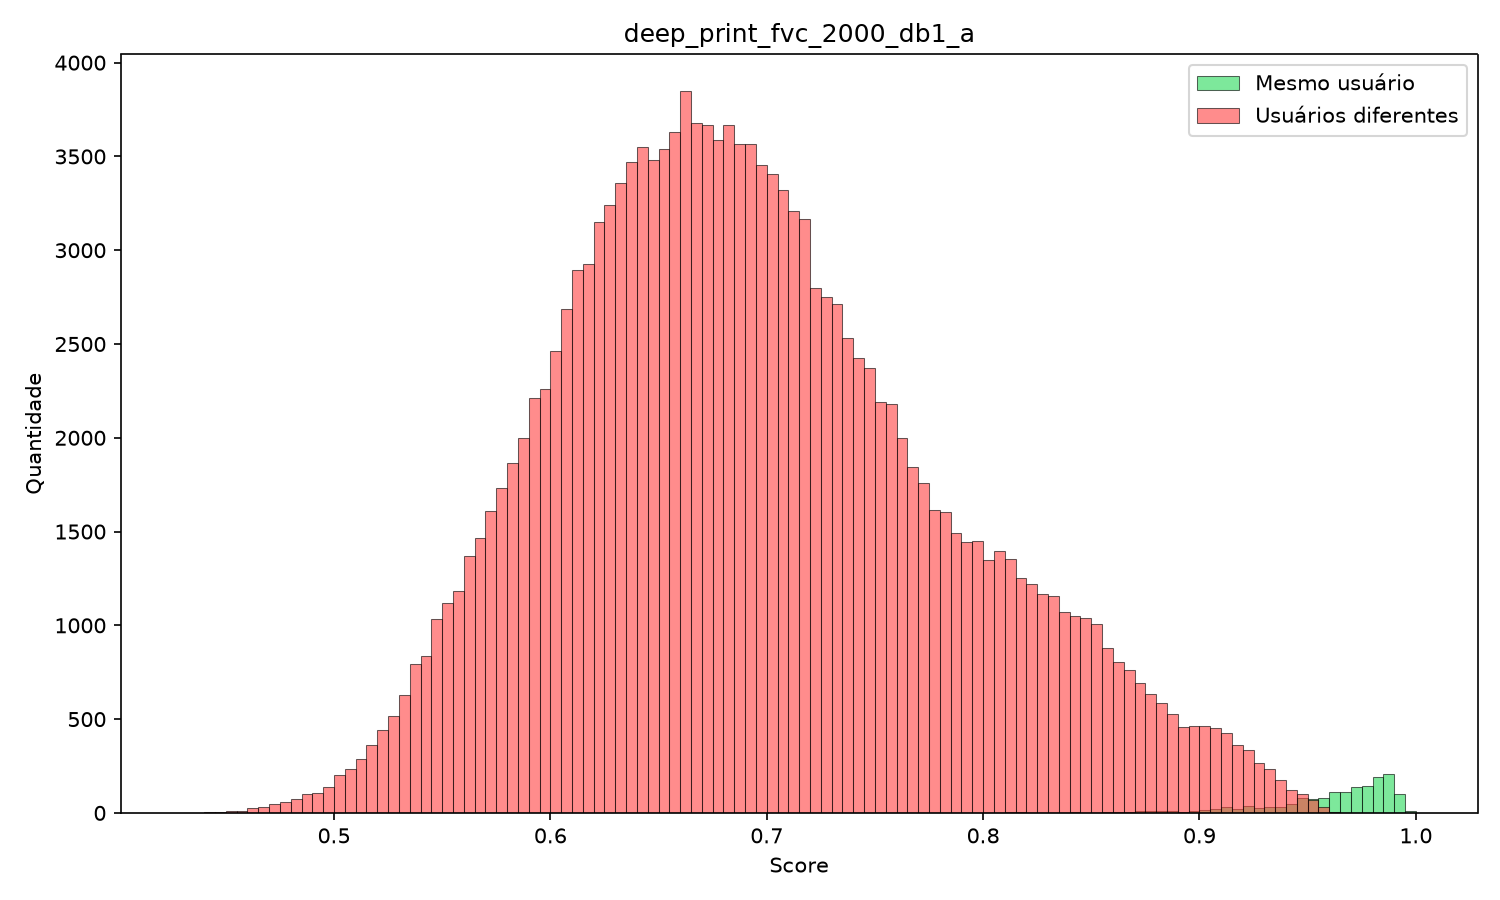
\includegraphics[width=\linewidth]{figures/results/deep_print_fvc_2000_db1_a.png}\\[0.15cm]
      {\fontsize{14.5pt}{18pt}\selectfont (a) DeepPrint -- DB1-A ($EER = 3,36\%$)}
    \end{minipage}\hfill
    \begin{minipage}[b]{0.32\linewidth}
      \centering
      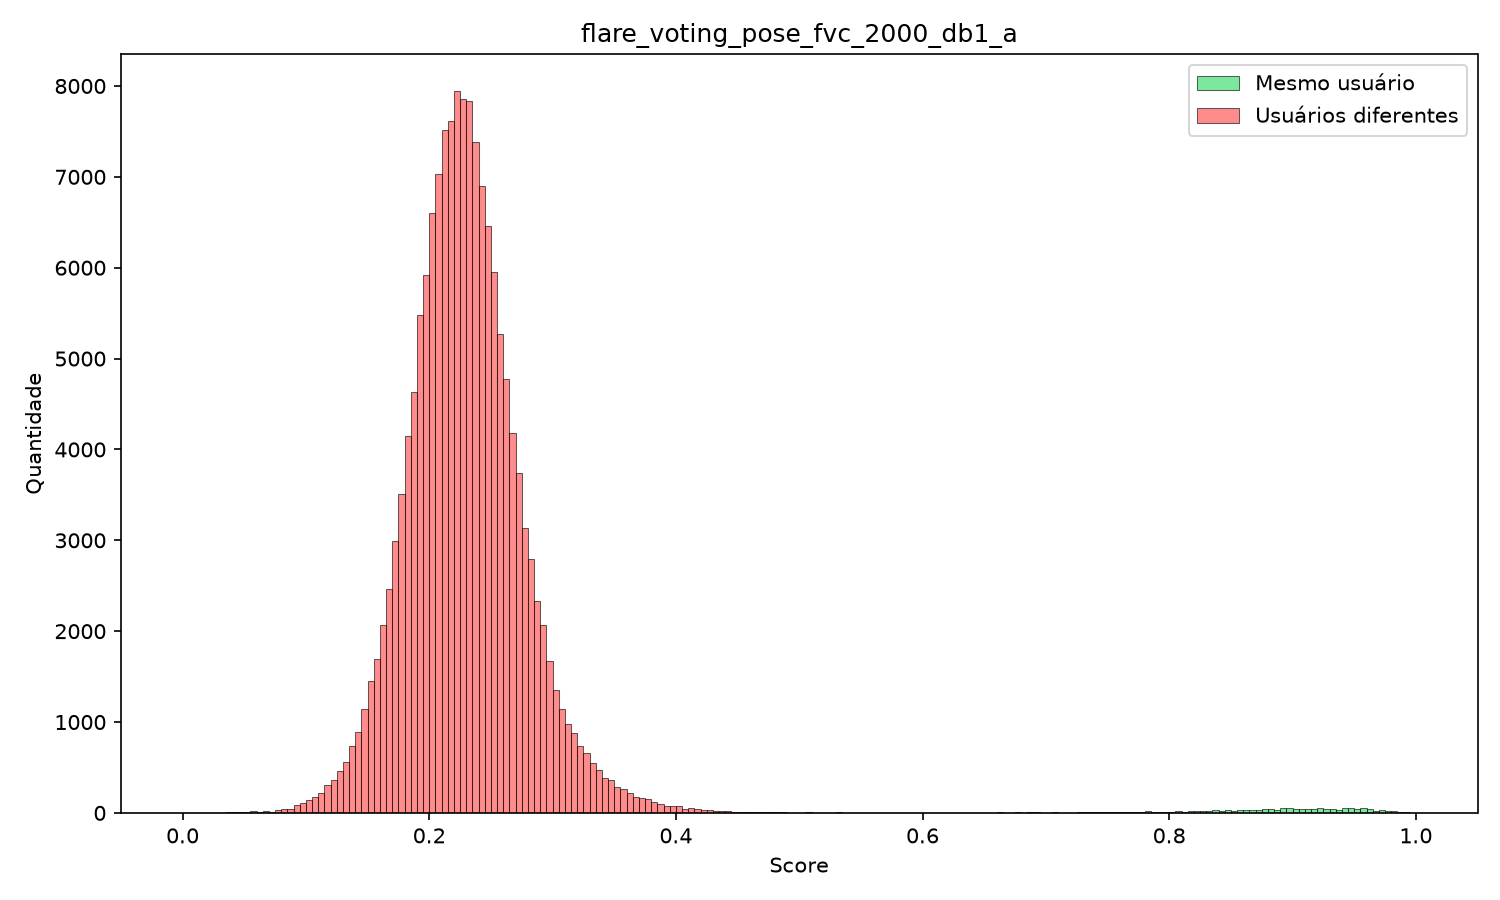
\includegraphics[width=\linewidth]{figures/results/flare_voting_pose_fvc_2000_db1_a.png}\\[0.15cm]
      {\fontsize{14.5pt}{18pt}\selectfont (b) FLARE Vot. -- DB1-A ($EER = 0,81\%$)}
    \end{minipage}\hfill
    \begin{minipage}[b]{0.32\linewidth}
      \centering
      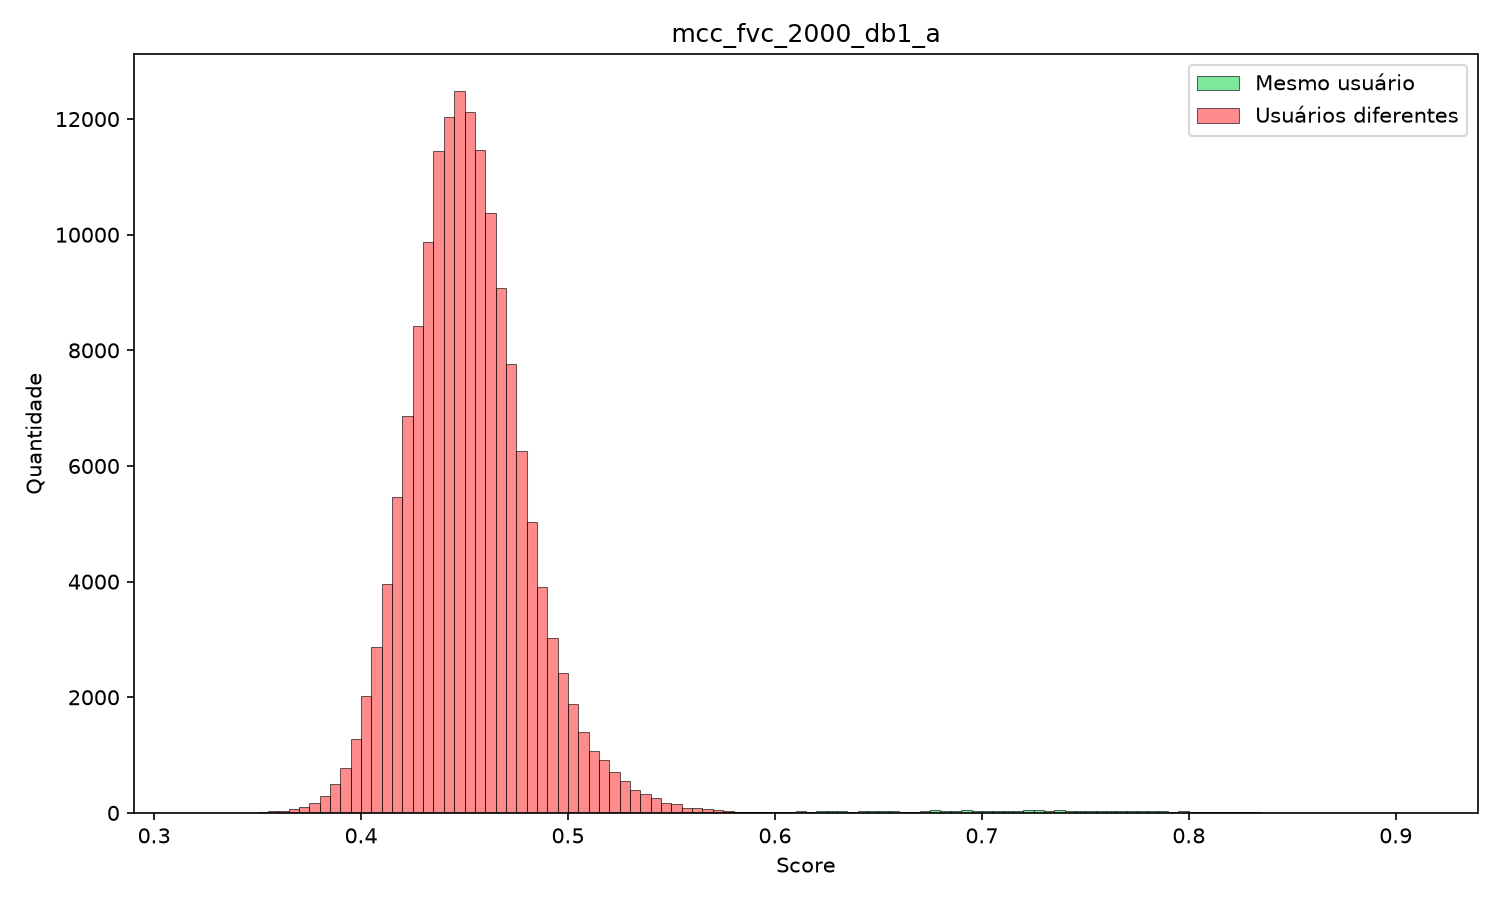
\includegraphics[width=\linewidth]{figures/results/mcc_fvc_2000_db1_a.png}\\[0.15cm]
      {\fontsize{14.5pt}{18pt}\selectfont (c) MCC -- DB1-A ($EER = 2,69\%$)}
    \end{minipage}\\[0.35cm]
    % Linha 2: Neurotechnology CrossMatch
    \begin{minipage}[b]{0.32\linewidth}
      \centering
      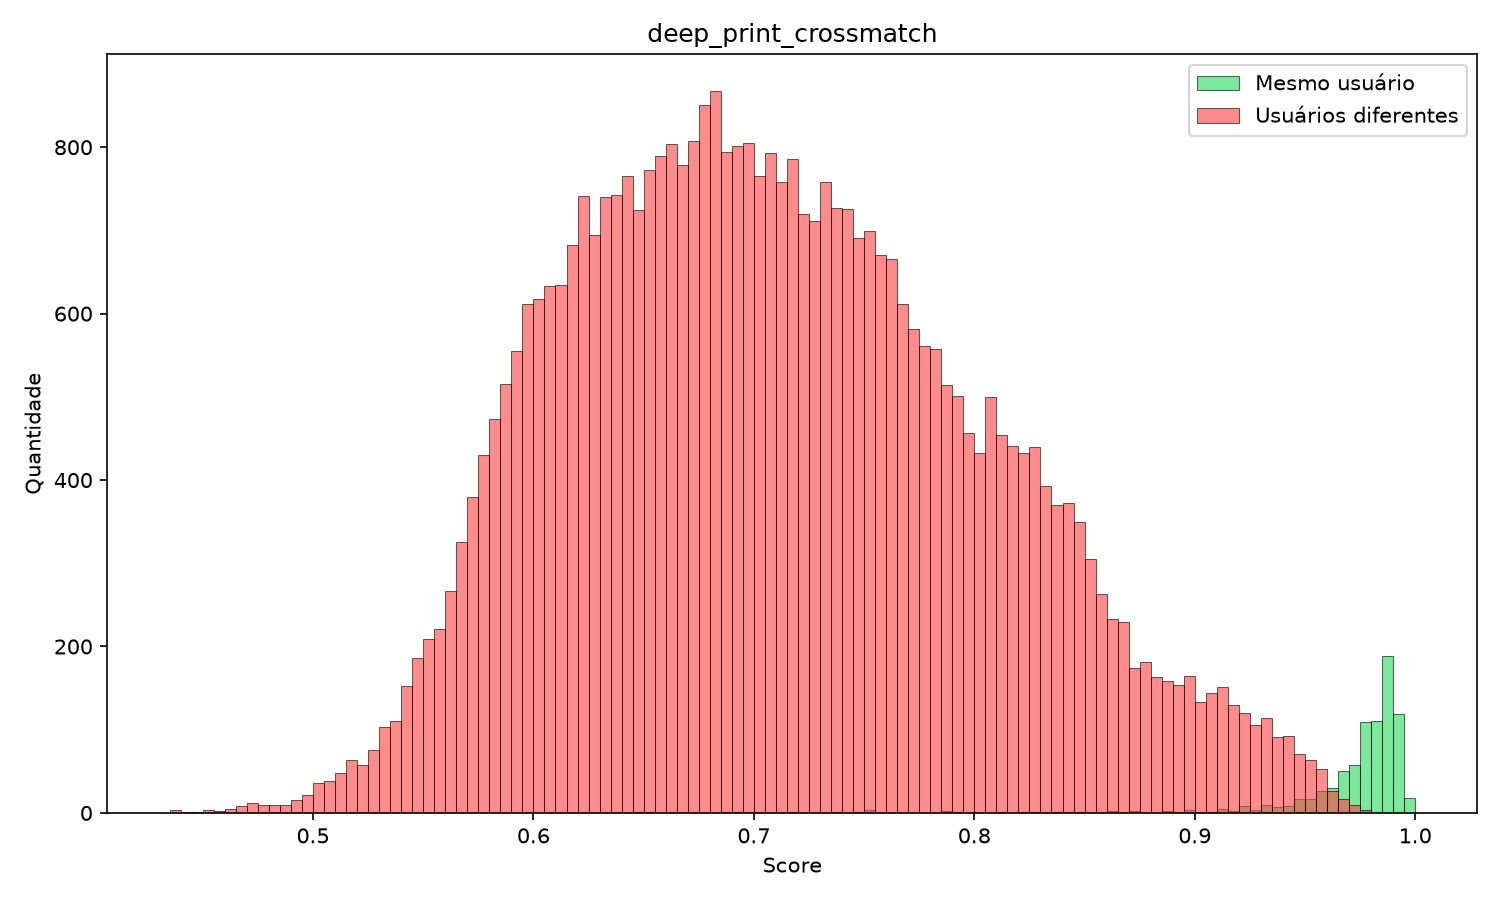
\includegraphics[width=\linewidth]{figures/results/deep_print_crossmatch.png}\\[0.15cm]
      {\fontsize{14.5pt}{18pt}\selectfont (d) DeepPrint -- CrossMatch ($EER = 3,31\%$)}
    \end{minipage}\hfill
    \begin{minipage}[b]{0.32\linewidth}
      \centering
      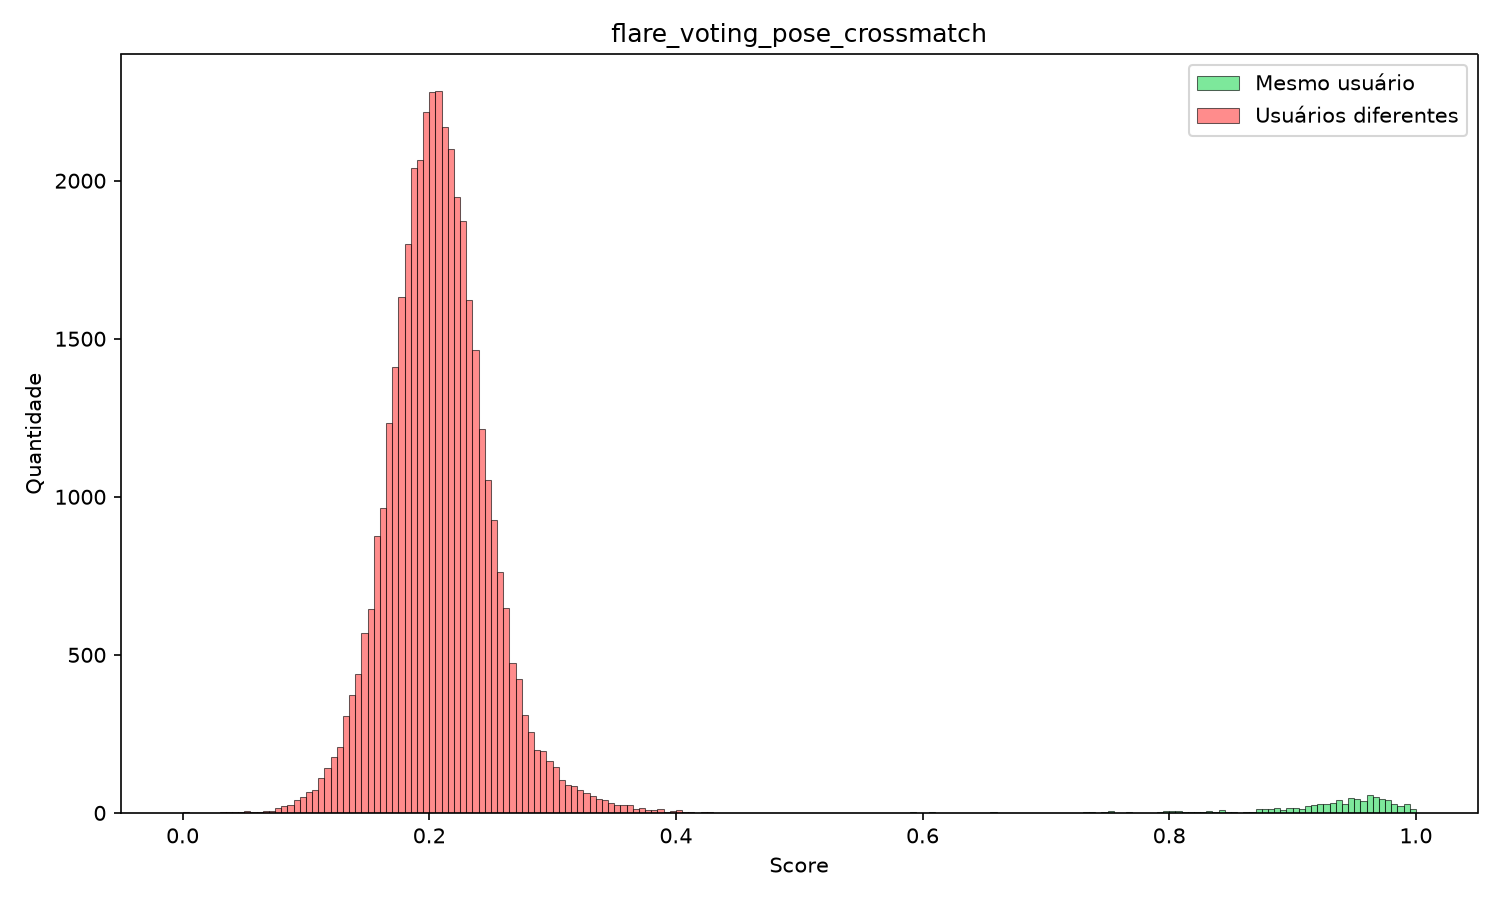
\includegraphics[width=\linewidth]{figures/results/flare_voting_pose_crossmatch.png}\\[0.15cm]
      {\fontsize{14.5pt}{18pt}\selectfont (e) FLARE Vot. -- CrossMatch ($EER = 0,12\%$)}
    \end{minipage}\hfill
    \begin{minipage}[b]{0.32\linewidth}
      \centering
      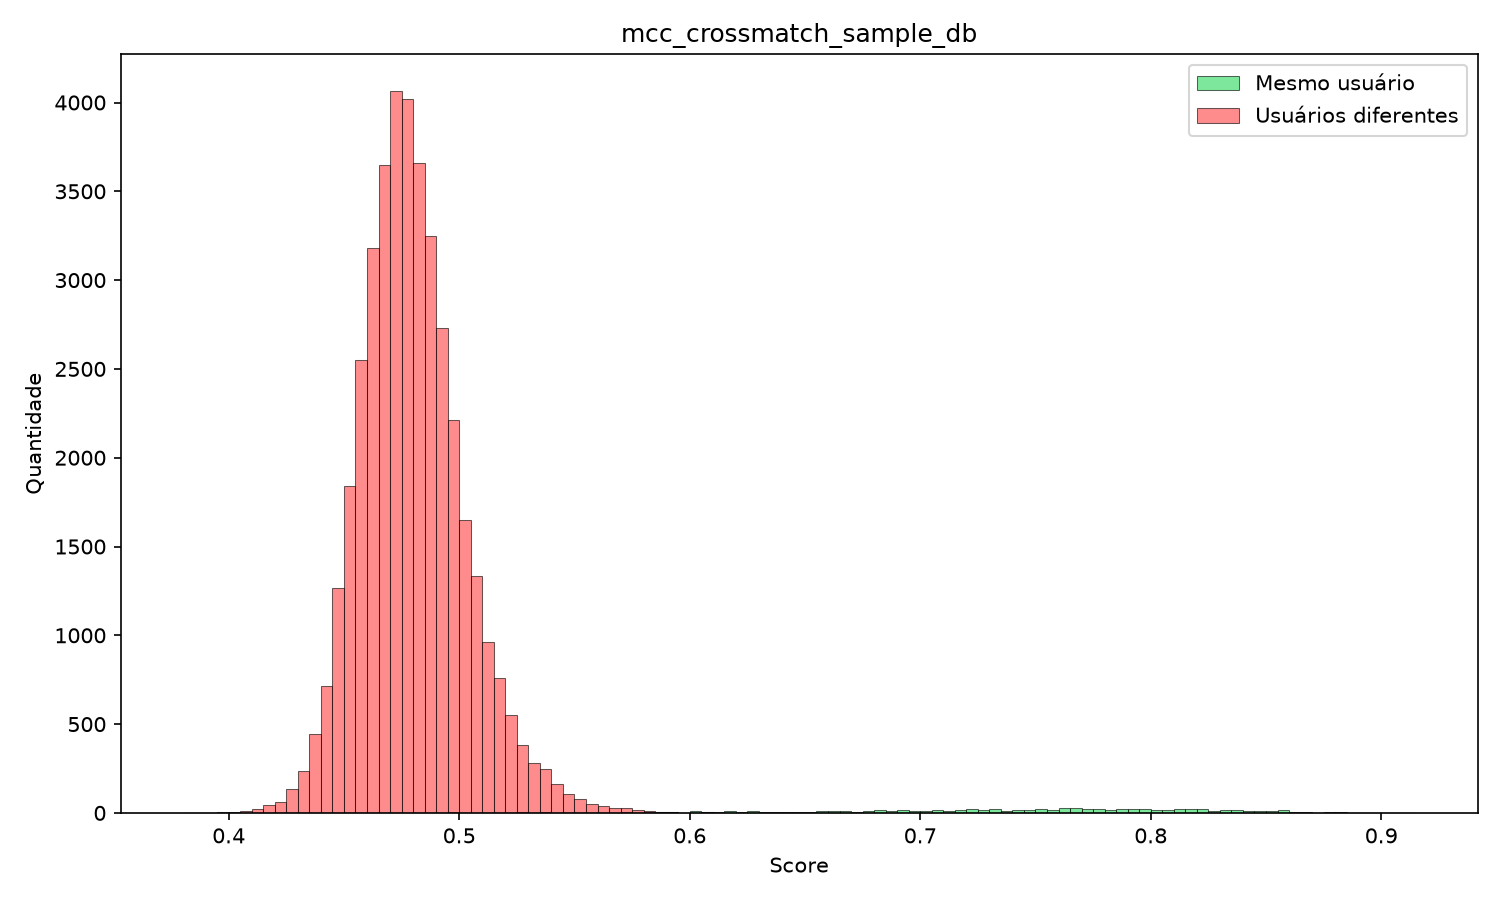
\includegraphics[width=\linewidth]{figures/results/mcc_crossmatch_sample_db.png}\\[0.15cm]
      {\fontsize{14.5pt}{18pt}\selectfont (f) MCC -- CrossMatch ($EER = 2,10\%$)}
    \end{minipage}\\[0.35cm]
    {\fontsize{18.5pt}{24pt}\selectfont \textbf{Figura 1:} Distribuição das pontuações de similaridade (Genuínos em verde vs Impostores em vermelho) para FVC2000 DB1-A e Neurotechnology CrossMatch.}
  \end{center}

  \vfill
  \postersection{CONCLUSÕES}
  \begin{itemize}[leftmargin=1.5cm, itemsep=0.4cm, topsep=0.3cm]
    \item O FLARE apresentou desempenho superior em todos os cenários avaliados, beneficiado pela retenção de relações geométricas espaciais e supressão explícita do fundo pela máscara de segmentação;
    \item O MCC exibiu excelente acurácia em impressões ópticas de alta qualidade, porém sua dependência estrita de minúcias torna-o vulnerável à degradação da imagem;
    \item O DeepPrint viabilizou alta velocidade de processamento com vetores 1D compactos, mas apresentou maior sensibilidade a ruídos severos devido à agregação global precoce;
    \item Etapas prévias de realce (UNetEnh e PriorEnh) não geraram aprimoramentos consistentes, evidenciando a robustez intrínseca das representações densas profundas.
  \end{itemize}

  \vfill
  \postersection{AGRADECIMENTOS}
  O presente trabalho foi realizado com apoio financeiro do \textbf{Conselho Nacional de Desenvolvimento Científico e Tecnológico (CNPq)} por meio de bolsa de Iniciação Científica, e da \textbf{Universidade Federal do ABC (UFABC)}.

  \vfill
  \postersection{REFERÊNCIAS}
  \fontsize{15.5pt}{21pt}\selectfont
  \noindent
  [1] ENGELSMA, J. J. et al. Learning a fixed-length fingerprint representation. \textit{IEEE TPAMI}, v. 43, n. 6, p. 1981--1997, 2021.\\[0.14cm]
  [2] YU, Y. et al. Dense representation for robust fixed-length fingerprint matching. \textit{IEEE TBIOM}, 2024.\\[0.14cm]
  [3] CAPPELLI, R. et al. Minutia Cylinder-Code: A new representation and matching technique. \textit{IEEE TPAMI}, v. 32, n. 12, p. 2128--2141, 2010.\\[0.14cm]
  [4] MALTONI, D. et al. \textit{Handbook of Fingerprint Recognition}. 2. ed. Springer, 2009.\\[0.14cm]
  [5] ROHWEDDER, T. DeepPrint: Evaluation of fixed-length fingerprint extractors. \textit{Master's Thesis}, Hasso Plattner Institute, 2023.

\end{minipage}

\end{document}
